% !TeX root = bericht.tex
\section{Aufgabe 1 - Regelstrecke}
\subsection{Signalflussbild}
\label{subsec:signalflussbild}
Der Elektromotor kann durch folgende Gleichungen beschrieben werden:
\begin{align}
    u(t)                       & = R \cdot i + L \cdot \frac{di}{dt} + K \cdot \omega \\
    M                          & = K \cdot i                                          \\
    J \cdot \frac{d\omega}{dt} & = M
\end{align}
Um das Signalflussbild zu zeichnen, müssen wir die Gleichungen nach den differenziellen Größen umstellen. Wir erhalten:
\begin{align}
    \frac{di}{dt}      & = \frac{1}{L} \cdot (u - R \cdot i - K \cdot \omega) \\
    \frac{d\omega}{dt} & = \frac{K}{J} \cdot i
\end{align}
Jetzt müssen wir nur noch zwei Integrator-Blöcke hinzufügen, um die Integrationen durchzuführen. 
Das Signalflussbild sieht dann wie folgt aus:
\begin{figure}[H]
    \centering
    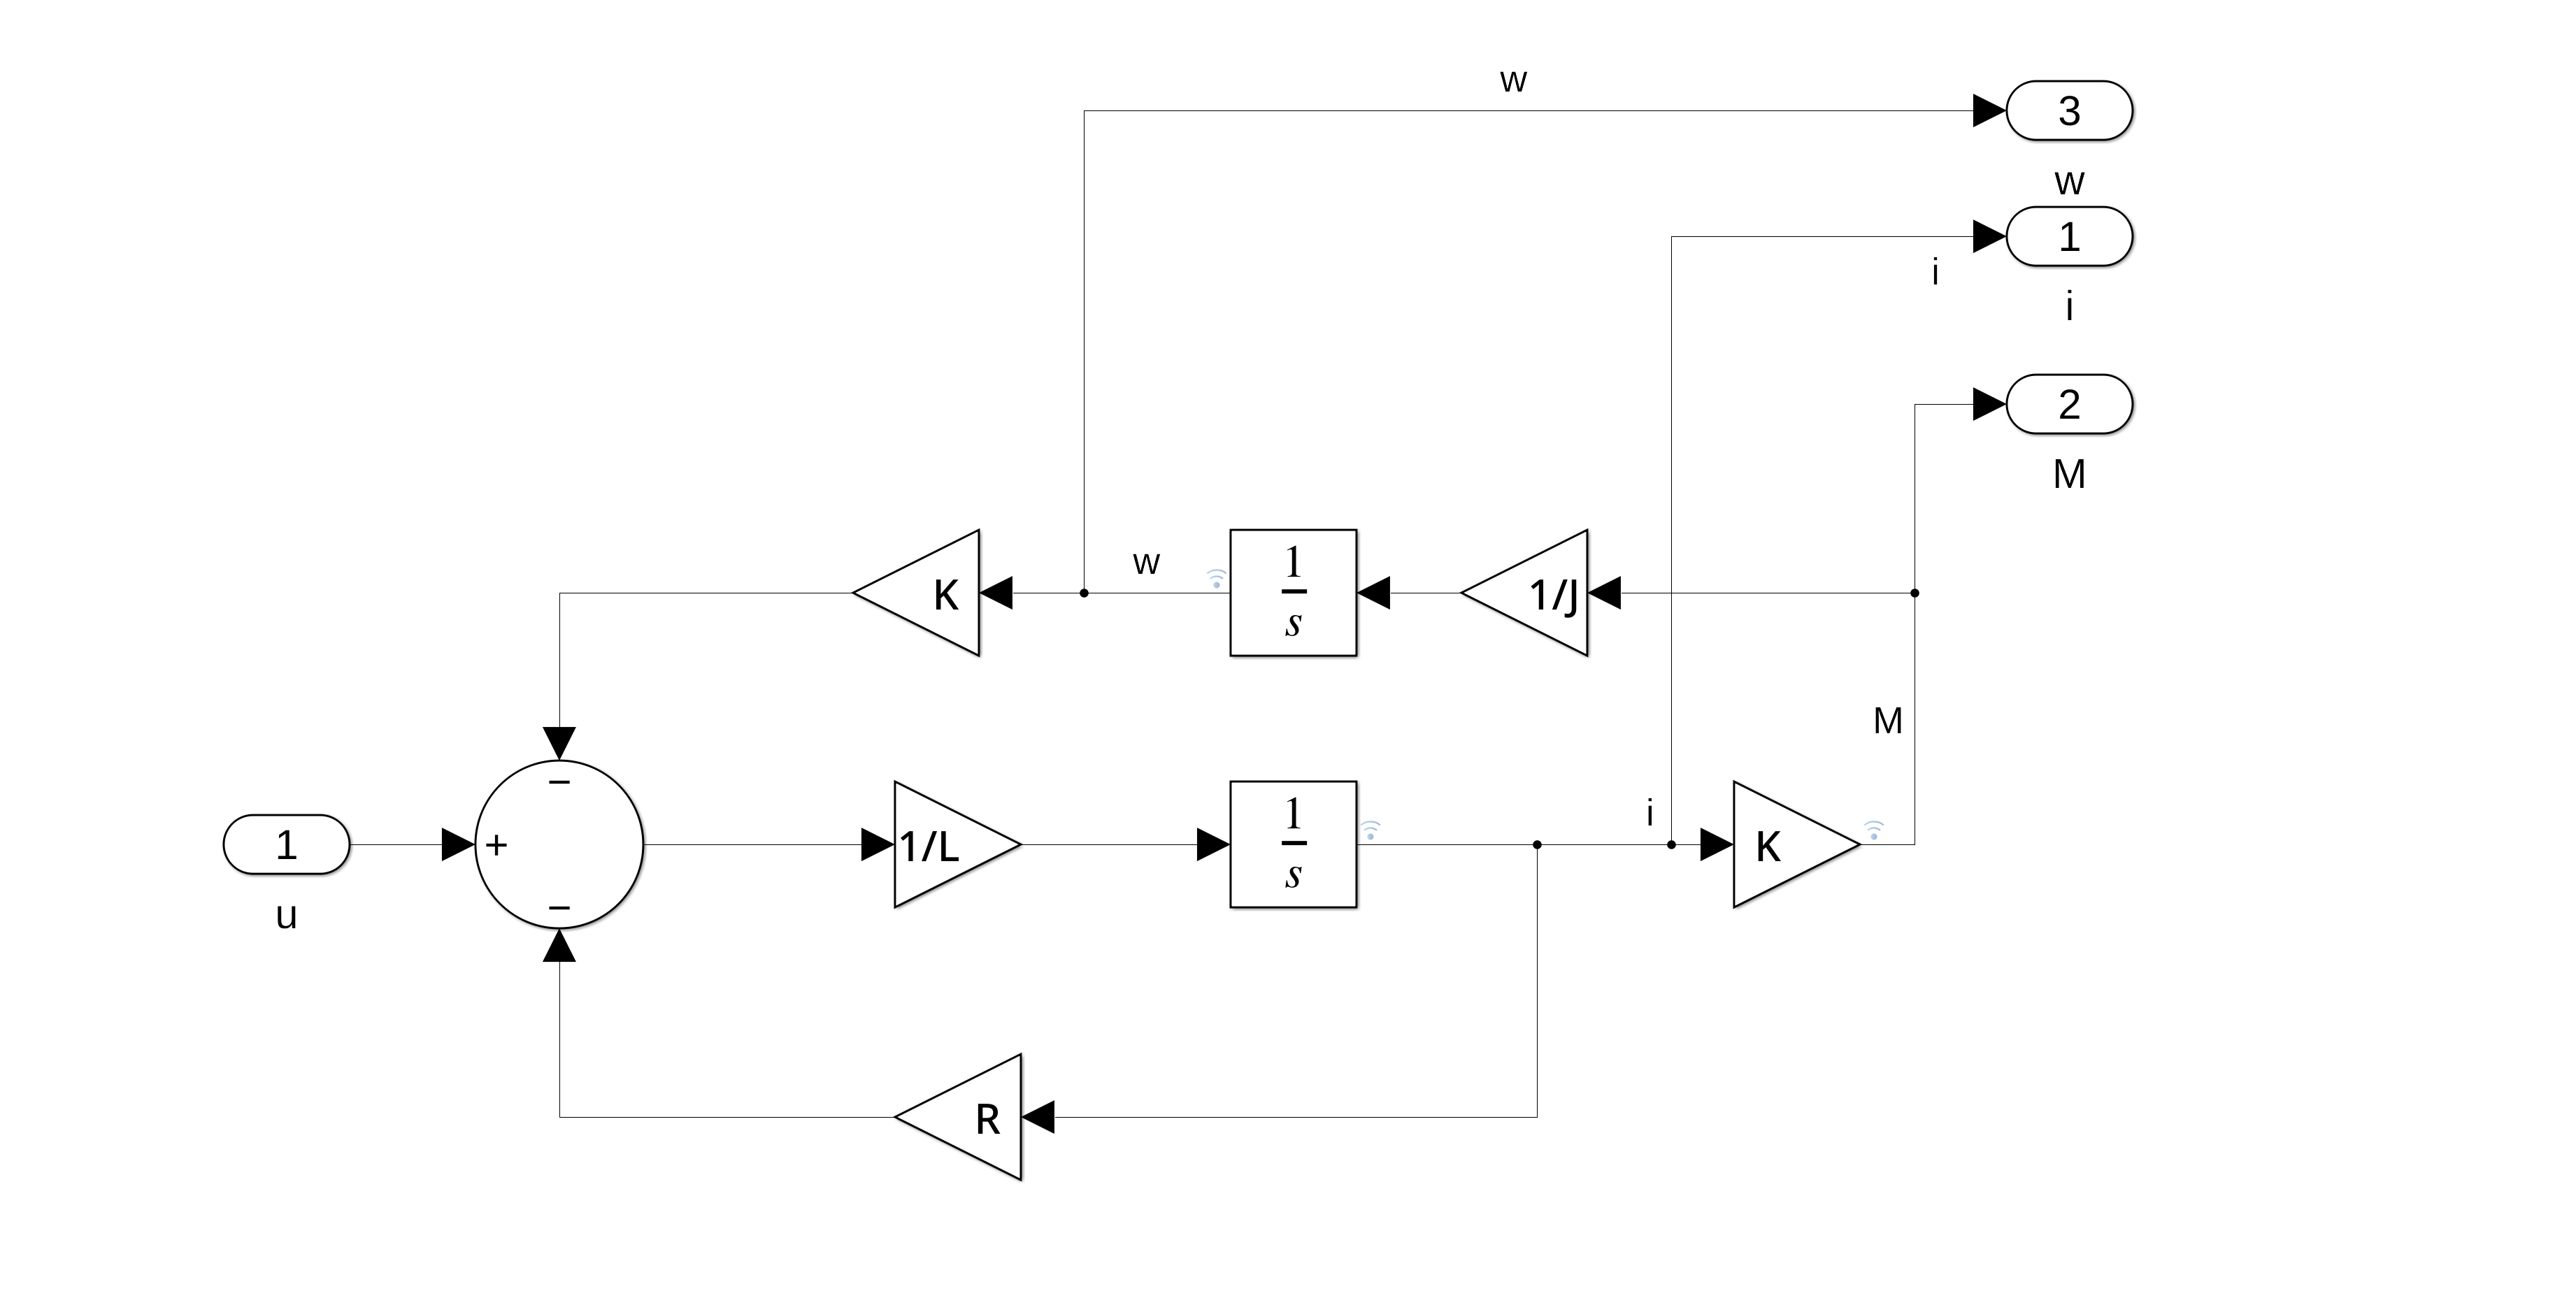
\includegraphics[width=1.0\textwidth]{images/Regelstrecke_simulink.png}
    \caption{Signalflussbild des Elektromotors}
\end{figure}
Für das Signalflussbild wurden die folgenden Parameter verwendet:
% K=30e-3; % in Nm/A; 30 mN*m/A
% J = 4e-4; % in kg*m^2; 4000 g*cm^2
% R=6; % in ohm; 6 Ohm
% L=120e-6; % in H; 120µH
\begin{itemize}
    \item $R = 6 \, \Omega$
    \item $L = 120 \, \mu H$
    \item $K = 30 \, mNm/A$
    \item $J = 4000 \, g \cdot cm^2$
\end{itemize}

\subsection{Simulation mit Simulink}
\begin{figure}[H]
    \centering
    
\includegraphics[width=1.0\textwidth]{regelstrecke_sim.png}
    \caption{Simulink Modell der Regelstrecke}
\end{figure}
Die Regelstrecke wurde in Simulink für 20s simuliert. 
Als Eingangssignal wurde ein Sprung von 0V auf 10V bei $t=0s$ verwendet.

\begin{sourcecode}[H]
    \caption{\textit{Matlab}-Code zur Simulation}
    \begin{minted}{matlab}
% ---------------- params for Regelstrecke Simulation ----------------
% step block parameters for Regelstrecke
init_value = 0; % initial value 0V
final_value = 10; % final value 10V
step_time = 0; % jump at 1s
sample_time = 0;
\end{minted}
\end{sourcecode}

Um die Simulation durchzuführen, wurde in einem MATLAB-Skript die Simulink-Funktion \texttt{sim} verwendet, um das Simulink-Modell zu starten.
Die Simulationsergebnisse wurden dann extrahiert, skaliert und in einem Diagramm geplottet.

\begin{sourcecode}[H]
    \caption{\textit{Matlab}-Code zur Simulation}
    \begin{minted}{matlab}
% load parameters
params;
disp('Parameters loaded');

% simulate using simulink model
sim_outputs = sim('regelstrecke_simulink', 'StopTime', '20');
disp('Simulation completed.');

% extract data from simulink
y_i = sim_outputs.logsout.get('i').Values; % Strmo extrahieren
y_u = sim_outputs.logsout.get('u').Values; % Eingang (Spannung) extrahieren
y_w = sim_outputs.logsout.get('w').Values; % Drehzahl extrahieren
y_M = sim_outputs.logsout.get('M').Values; % Drehmoment extrahieren

% change units
% y_w.Data = y_w.Data * (60/(2*pi)); % convert rad/s to rpm
y_M.Data = y_M.Data * 1e3; % convert Nm to mNm
y_i.Data = y_i.Data * 10; % convert A to 10 mA

% plot results in one plot
figure('Name', 'Simulation der Regelstrecke');
hold on;
grid on;
plot(y_i.Time, y_i.Data, 'b', 'LineWidth', 1.5);
plot(y_M.Time, y_M.Data, 'r', 'LineWidth', 1.5);
plot(y_w.Time, y_w.Data, 'g', 'LineWidth', 1.5);
ylabel('Werte');
xlabel('Zeit [s]');
legend('Strom i [10 mA]', 'Moment M [mNm]', 'Drehzahl w [rad/s]', 'Location', 'best');
title('Simulationsergebnisse der Regelstrecke');
hold off;

% export plot
exportgraphics(gcf, './lab3/images/a1_regelstrecke_sim.png', 'Resolution', 300);
    \end{minted}
\end{sourcecode}

Daraus erhalten wir die folgenden Simulationsergebnisse:
\begin{figure}[H]
    \centering
    
\includegraphics[width=0.9\textwidth]{a1_regelstrecke_sim.png}
    \caption{Simulationsergebnisse der Regelstrecke}
\end{figure}

Man sieht hier, dass unser Motor eine maximale Drehzahl von ca. 322 rad/s erreciht.
Dies ist das Eigenverhalten von unserem Motor.

\subsection{Zeitkonstante}
\label{sub:regelstrecke_tau}
Die Zeitkonstante $\tau$ der Regelstrecke kann aus der Simulationsergebnisse berechnet werden.
\begin{sourcecode}[H]
    \caption{\textit{Matlab}-Code zur Berechnung der Zeitkonstante}
    \begin{minted}{matlab}
endwert = y_w.Data(end); % Endwert der Drehzahl
gesuchter_wert = 0.63 * endwert; % 63% des Endwerts
index_63 = find(y_w.Data <= gesuchter_wert, 1); % Index des ersten Werts <=63% des Endwerts
zeit_63 = y_w.Time(index_63); % Zeit bei 63% des Endwerts
tau = zeit_63 - step_time; % Zeitkonstante tau
disp(['Zeitkonstante tau: ', num2str(tau), ' Sekunden']);
    \end{minted}
\end{sourcecode}

\begin{consoleoutput}[H]
    \centering
    \caption{Zeitkonstante der Regelstrecke}
    \begin{minted}[linenos=false]{text}
Zeitkonstante tau: 3.0365 Sekunden
    \end{minted}
\end{consoleoutput}